\label{cap:solucion}

Una vez vistas todas las alternativas para cada caso en el capítulo anterior, es necesario elegir las alternativas que se adapten más a la solución pretendida para este Proyecto.

\section{Diseño de arquitectura de la solución}

    En la figura~\ref{diagrama_bloques} se observa el diagrama de bloques del sistema. El timbre conecta con el nodo central a través de un sistema de interconexión. El telefonillo conecta de la misma manera con el nodo central, a través de otro sistema de interconexión. A su vez, el nodo central se conecta al smartphone y a los nodos informativos visuales a través de un sistema de comunicación. Es necesario considerar este diagrama de bloques a lo largo de la exposición de la solución propuesta, para entender todo el conjunto que conforma el sistema final. \\

    \begin{figure}[H]
      \centering
        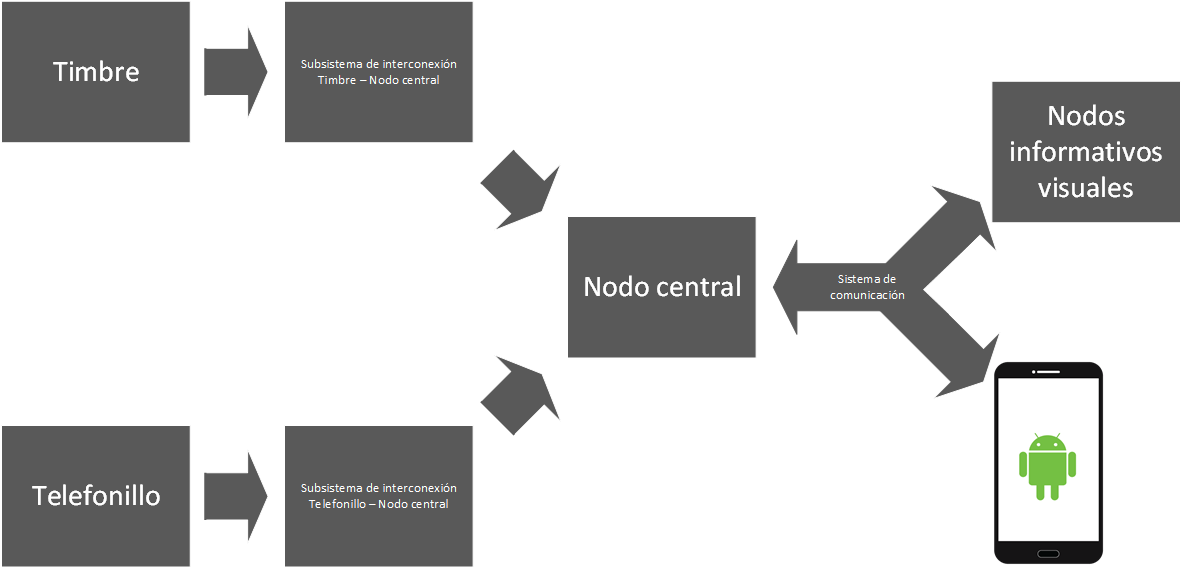
\includegraphics[width=1\textwidth]{diagrama_bloques.png}
      \caption{Diagrama de bloques del sistema.}
      \label{diagrama_bloques}
    \end{figure}

\section{Elección de los nodos informativos visuales}
    \label{sec:solucionbombillas}

    Teniendo en cuenta la tabla~\ref{tab:bombillas}, a raíz del estudio de Requisitos dentro de las Especificaciones del Sistema [~\ref{sec:especificaciones}], y sobre todo, de acuerdo con el requisito no funcional NFR-01, se busca utilizar bombillas capaces de generar luces de colores (RGB), la segunda alternativa mostrada en la tabla queda descartada, pues tan solo proporciona luz en distintos tonos de blanco (ya sea luz más cálida o más fría, y variaciones de luminosidad). \\

    Además, la tercera opción expuesta podría resultar a primera vista la solución más económica, pues permite la compra por separado del puente que comunica con las bombillas, pero debido a ser compra en el extranjero, con importantes gastos de transporte, y la imposibilidad de facturar estos gastos a través de la universidad, se descarta también esta opción. \\

    Queda claro por tanto que la opción elegida es la primera, utilizar las bombillas Hue de Philips. Estas bombillas utilizan un puente ZigBee-Ethernet, al que se conecta mediante cable Ethernet y se utiliza una interfaz propia para alterar el estado de las bombillas. Estas se controlan mediante métodos HTTP a través de una interfaz RESTful, los cuales deben recibir y generar cadenas en formato JSON, por lo que es necesario poder manipular estas cadenas de alguna manera.

\section{Elección de dispositivo de interconexión de red}

    Se ha visto la necesidad de conectar un smartphone Android al sistema (según el requisito no funcional NFR-02), y la solución más acertada para la conexión de este dispositivo parece WiFi, ya que como se ha visto, tiene mayor alcance que Bluetooth, pudiendo funcionar por tanto mucho mejor en el entorno del interior de una vivienda (teniendo en cuenta las paredes que se encuentran dentro de una vivienda). \\

    Con Bluetooth, se tiene un alcance de 10 metros, 100 en condiciones óptimas (sin obstáculos) y mediante el uso de repetidores. Con WiFi, el alcance es mucho mayor, llegando a 70-100 metros en interior, y hasta 250 metros en condiciones óptimas (en exteriores). Siendo estas dos las únicas opciones de conexión posibles para un smartphone Android, queda descartado el uso de Bluetooth, eligiendo así utilizar WiFi como medio de comunicación. \\

    Es necesario por tanto el uso de un punto de acceso WiFi al que el smartphone Android pueda conectar, comunicando así el smartphone y el nodo central. Además, para la conexión del nodo central con el puente Hue utilizado para la comunicación con las bombillas elegidas, es necesario el uso de un dispositivo que realice la función de un switch Ethernet. Debido a estas necesidades y teniendo en cuenta lo expuesto en el apartado~\ref{sec:routerintegrado} del Informe de Diagnóstico, en el que se explica que habitualmente dentro de una vivienda se cuenta con un dispositivo que cumple con estas características (un router integrado)\cite{cisco_ccna}, se decide utilizar este dispositivo para la interconexión de los tres sistemas: el nodo central, el smartphone y el puente Hue.\\

    Tanto Arduino como Raspberry Pi, las dos opciones analizadas para utilizar como nodo central, pueden lograr conexión a la red mediante un latiguillo Ethernet como solución más simple, necesitando Arduino de una placa Ethernet para lograr la conexión.

\section{Elección del nodo central}

    Tras descartar Arduino como placa programable que funcionase como nodo central, se decidió continuar con la otra alternativa estudiada: utilizar una Raspberry Pi B como nodo central. \\

    En la Raspberry Pi B se cuenta ya con interfaz de red Ethernet, por lo que no es necesario utilizar ninguna placa añadida. Además esta placa también cuenta con pines de entrada/salida programables, lo cual es indispensable para el desarrollo del Proyecto. \\

\section{Aplicación para nodo central}

    Se utilizará Python como lenguaje de programación para los programas del sistema, lenguaje cada vez más utilizado en proyectos de este tipo en los que se necesita dotar a Raspberry Pi de funcionamiento junto a sensores y otros sistemas hardware. Además, Python incluye librerías que permiten manejar cadenas JSON, establecer comunicaciones mediante peticiones HTTP, y más. Se utilizará la implementación 2.7 de Python, con soporte para todas las librerías necesarias en el Proyecto, como son las de manejo de direcciones URL.\\

    Es necesario además instalar en el sistema operativo la librería RPi.GPIO, librería externa facilitada por Python para el manejo de los pines GPIO de Raspberry Pi, necesario para la lectura del estado de los relés empleados para la detección de llamadas al telefonillo o al timbre. \\


    \subsection{Librerías desarrolladas}

        Se ha desarrollado por tanto un conjunto de programas que sean capaces de comunicarse con el puente Philips Hue mediante métodos REST y cadenas JSON (utilizadas tanto para parámetros como para respuestas del puente), detectar las alertas de las llamadas entrantes tanto de telefonillo como de timbre a través de los relés empleados para ello, y comunicarse con un dispositivo Android para replicar las mismas alertas, a modo de texto. \\
        
        Se desarrollan para ello dos librerías en Python: una para el uso de métodos REST, y otra para el control del puente Philips Hue. \\

        \subsubsection{Librería RESTful}

        Para ello, se ha desarrollado en primer lugar una librería REST en Python, que facilita la comunicación de Raspberry Pi con el puente Philips Hue. Esta librería, implementada en un único fichero, cuenta con 4 métodos principales, que serán los utilizados por el usuario: \textbf{get, post, put} y \textbf{delete}. Cada uno de ellos recibe la dirección del dispositivo al que realizar la petición, el dato a utilizar en caso de que sea necesario (POST y PUT), y el tipo de contenido del mensaje, que en este caso será siempre texto formateado en JSON. \\

        \pythonexternal[linerange={4-7,11-12,56-67}]{./contenido/src/raspberry/rest.py}
        \vspace{0.3cm}
        Además, la misma clase de la librería cuenta con un método genérico privado el cual utilizan las 4 funciones anteriores. Este método es el verdadero encargado de establecer la conexión con el dispositivo deseado, y realizar la petición REST proporcionando además los datos que sean necesarios, y recogiendo la respuesta proporcionada por el dispositivo en formato JSON. \\

        \pythonexternal[linerange={13-13,22-55}]{./contenido/src/raspberry/rest.py}
        \vspace{0.3cm}
        Lo primero que hace este método es comprobar si hay datos entrantes, si los hay, los formatea como JSON mediante la librería propia de Python, y luego comprueba el tipo de petición (PUT o POST, las dos peticiones que pueden recibir datos entrantes). \\

        Para efectuar el PUT, establece la conexión utilizando la dirección recibida, añade los datos a enviar, y la cabecera con el tipo de contenido. Finalmente realiza la petición. Por otro lado, para POST, se distinguen dos tipos: con y sin cuerpo del mensaje. Se realizan los mismos pasos, salvo que efectuando una petición POST. \\

        En cambio, si no hay datos entrantes, la petición podrá ser GET o DELETE. Se realizan las mismas acciones que en el caso anterior, solo que sin incluir datos en la petición. Finalmente, se almacena la respuesta, se cierra la conexión y se devuelve la respuesta. \\

        \subsubsection{Librería Hue}

        Por otra parte, se ha creado una librería Python para el control del puente Philips Hue, así como de las bombillas asociadas a él. Gracias a esta librería, se evita utilizar la interfaz web propia del puente, que únicamente debe utilizarse como herramienta para desarrolladores, en concreto para depuración y pruebas. Esta librería se divide en tres clases:
        \begin{itemize}
            \item Bridge: clase principal, de la que se debe crear un objeto para poder utilizar el sistema. Contendrá información como el usuario del puente Philips Hue a utilizar, o la dirección IP del mismo.
            \item Light: clase que implementa todas las funciones necesarias para el control de las bombillas, como obtener su estado o modificarlo.
            \item Config: clase que contiene funciones necesarias para la configuración del puente Philips Hue desde el mismo programa, sin necesidad de acceder a la interfaz web de depuración.
        \end{itemize}

        Estas clases están repartidas en distintos archivos.

        \paragraph{Clase Bridge}\mbox{}\\

        La clase principal de la librería está implementada en el fichero \_\_init\_\_.py del paquete de la librería, siguiendo las directrices de Python para la implementación de clases, métodos y otras funciones que se deseen ejecutar como inicialización de las librerías o paquetes creados. Esta clase principal, Bridge, cuenta únicamente con un constructor. \\

        \pythonexternal[linerange={4-14}]{./contenido/src/raspberry/__init__.py}
        \vspace{0.3cm}

        El constructor recibe la dirección IP del puente y el nombre del usuario del puente a utilizar, crea un objeto de cada una de las otras clases, Config y Light, utilizando estos parámetros; y busca en la misma inicialización bombillas que hayan sido recientemente instaladas en la vivienda, para asociarlas al puente Hue.

        \paragraph{Clase Config}\mbox{}\\

        La clase Config únicamente contiene 3 métodos relacionados con la configuración y estado del puente. Esta clase además, utiliza la librería REST anteriormente expuesta, para la comunicación con el puente. \\

        \pythonexternal[linerange={3-12,17-27}]{./contenido/src/raspberry/config.py}
        \vspace{0.3cm}

        Obviando el constructor, el cual es trivial, el primero de los métodos es un observador que comprueba si se puede conectar al puente con el usuario dado, o por el contrario, es un usuario no autorizado a utilizar dicho dispositivo. Este método realiza una petición GET a la dirección ``\textit{http://IP\_PUENTE/api/USUARIO}'', recibiendo como respuesta una cadena JSON con toda la configuración del puente si el usuario está autorizado, o un error si el usuario no está dentro de la lista de usuarios autorizados a realizar operaciones con el puente. \\

        \pythonexternal[linerange={29-29,35-39}]{./contenido/src/raspberry/config.py}
        \vspace{0.3cm}

        El segundo método recibe una cadena con el nombre de un nuevo usuario, y crea un usuario en el puente con ese nombre. De nuevo, utilizando peticiones REST, en concreto POST, se realiza la operación, resultando una cadena JSON que informará si la operación se ha realizado con éxito. \\

        \pythonexternal[linerange={41-41,47-52}]{./contenido/src/raspberry/config.py}
        \vspace{0.3cm}

        Por último, el tercer método realiza justo lo contrario que el anterior: elimina un usuario de la lista de usuarios autorizados a utilizar el puente, recibiendo como parámetro el nombre del usuario a eliminar. Mediante una petición DELETE a la dirección necesaria, se elimina ese usuario, y se devuelve información relativa al resultado de la operación.

        \paragraph{Clase Light}\mbox{}\\

        La última clase de la librería Python para Hue es Light. Esta clase implementa las funciones necesarias para controlar las bombillas Hue, como son obtener el estado de las bombillas, el número de bombillas conectadas, el estado de una bombilla individual, encontrar nuevas bombillas que conectar al puente Hue, y diversos modificadores de su estado. \\

        \pythonexternal[linerange={4-12,17-37}]{./contenido/src/raspberry/light.py}
        \vspace{0.3cm}

        Al igual que en la clase Config, el constructor es bastante trivial. El primer método de interés que se encuentra es \textbf{get}, el cual se encarga de obtener del puente Philips Hue la información de todas las bombillas conectadas, las nuevas, o una única bombilla determinada, dependiendo de la información que reciba como parámetro. Una vez controlado de qué bombilla o bombillas debe obtener la información, realiza una petición GET, y devuelve el resultado de esta operación, exceptuando si debe obtener información de todas las bombillas, caso en el que reagrupa la información de las bombillas en un vector de bombillas (vector de información de cada una de las bombillas). \\

        \pythonexternal[linerange={39-39,44-52}]{./contenido/src/raspberry/light.py}
        \vspace{0.3cm}

        El método \textbf{getNumLights} se basa en el método anterior, y a diferencia de este no recibe parámetros. Este método realiza directamente una petición GET para obtener el estado de todas las bombillas conectadas al puente, para después transformar la respuesta en un vector de bombillas, y finalmente devolver la longitud de ese vector (o lo que es lo mismo, el número de bombillas). \\

        \pythonexternal[linerange={54-54,59-61,67-67}]{./contenido/src/raspberry/light.py}
        \vspace{0.3cm}

        Los siguientes métodos, \textbf{getLightState} y \textbf{isPhisicallyOn} reciben como parámetro el número identificador de una bombilla, y utilizan internamente el método \textbf{get} expuesto anteriormente. El primero, filtra la salida de \textbf{get}, devolviendo únicamente el campo \textbf{state} del JSON generado. El segundo, hace lo mismo y además se queda solo con el parámetro \textbf{reachable} de \textbf{state}, el cual determinar si una bombilla está encendida físicamente o no (y no a través del puente Hue). \\

        \pythonexternal[linerange={69-69,73-77}]{./contenido/src/raspberry/light.py}
        \vspace{0.3cm}

        La función \textbf{findNewLights} realiza una operación parecida a \textbf{get}, cambiando que ejecuta una petición POST en lugar de GET. El resultado de realizar POST a la misma dirección mediante la cual se obtiene información de todas las bombillas con \textbf{get}, es buscar nuevas bombillas pendientes de conectar al puente, y asociarlas automáticamente a este. \\

        \pythonexternal[linerange={79-79,84-96}]{./contenido/src/raspberry/light.py}
        \vspace{0.3cm}

        Utilizado por los modificadores de estado como método base, el método \textbf{update} es un método genérico para modificar el estado de una bombilla conectada al puente Hue. Este método recibe un dato, y dependiendo de si ese dato es interno al parámetro \textbf{attr} o \textbf{state} de la bombilla, realiza la petición POST a distintas URL, junto al dato que se ha proporcionado. El resultado de este método es la modificación del estado de la bombilla, además de devolver información sobre la operación realizada. \\

        \pythonexternal[linerange={98-98,106-112,122-128,133-139,144-148}]{./contenido/src/raspberry/light.py}
        \vspace{0.3cm}

        Los últimos métodos de la clase, los modificadores de estado, son bastante simples, al utilizar internamente el método \textbf{update} genérico anterior. \textbf{setLightColor} recibe el identificador de una bombilla y los parámetros relacionados con el color, y realiza un \textbf{update} para modificar estos parámetros. \textbf{setLightState} realiza lo mismo y además, modifica también si la bombilla quedará encendida o apagada, recibiendo este atributo de estado como parámetro. Por otra parte, \textbf{setLightOn} y su contrapartida, \textbf{setLightOff} sirven para alterar el estado de encendido de la bombilla: encenderla y apagarla, respectivamente.

    \subsection{Programa principal}

        El programa principal del nodo central utiliza las librerías anteriores para conectar con el puente Philips y controlar las bombillas. Este programa además utiliza también varias librerías de Python como son \textbf{socket, sys, threading,} y la librería externa \textbf{RPi.GPIO}, entre otras.
        
        \subsubsection{Cabecera del programa y definición de variables globales}

        \pythonexternal[linerange={19-55}]{./contenido/src/raspberry/main.py}
        \vspace{0.3cm}

        En la primera parte del programa, se definen varias variables utilizadas a lo largo de este. Las cuatro primeras variables pueden modificarse, definiéndose en ellas el nombre de usuario a utilizar para conectar al puente, el idioma de los mensajes enviados al smartphone (español o inglés), y el número de los pines GPIO a los que se conectarán las señales del telefonillo y el timbre. \\

        El resto de variables definidas son variables de cadenas de caracteres en los distintos idiomas, el identificador Hue de los colores a utilizar para mostrar las alertas mediante las bombillas, la configuración de los pines GPIO, y el comando a utilizar para descubrir la dirección IP asociada al puente Hue de manera automática. Este último utiliza comandos de consola del sistema para obtener la dirección IP de la red a la que se está conectado mediante \textbf{ip route show} y varios \textbf{grep} (uno de ellos utilizando expresiones regulares para determinar el formato de la dirección IP), proporcionar ese comando a la herramienta de escaneo ARP \textbf{arp-scan}, la cual proporcionará la dirección IP de los dispositivos conectados a la red, filtrando por último el dispositivo de interés (el puente Philips Hue) para obtener únicamente su dirección IP mediante \textbf{awk}. Mientras no se obtenga la dirección del puente Hue como resultado y por tanto no se pueda conectar con él, el programa quedará iterando en estos comandos, a la espera de realizar la conexión.
        
        \subsubsection{Asociación de usuario al puente Philips Hue}

        \pythonexternal[linerange={57-69}]{./contenido/src/raspberry/main.py}
        \vspace{0.3cm}

        Entre los métodos de este programa se encuentra \textbf{linkUserConfig}, el cual se encarga de asociar el usuario configurado al puente Philips Hue si no estuviese ya creado y admitido dentro de la lista de usuarios con permisos para controlar el puente, mediante la función \textbf{createUser} de la clase Config.
        
        \subsubsection{Alerta mediante puente Philips Hue}

        \pythonexternal[linerange={71-94}]{./contenido/src/raspberry/main.py}
        \vspace{0.3cm}

        El método para mostrar las alertas a modo de parpadeo de luces de colores en las bombillas es \textbf{lightAlert}, el cual recibe el identificador de color de la alerta y comprueba si el usuario tiene permisos de conexión al puente mediante el método \textbf{isConnected} de la clase Config. Si no los tiene, se utilizará el método \textbf{linkUserConfig()} de este mismo programa. Además, al igual que se realiza al principio de la ejecución del programa al crear el objeto Bridge, se comprueba si se pueden asociar nuevas bombillas al puente Hue, para tener control en todo momento sobre todas las bombillas al alcance del puente. Tras esto se realiza una serie de operaciones para almacenar el estado previo de todas las bombillas conectadas al puente (mediante el método \textbf{getLightState} de la clase Light), cambia su estado a uno de encendido y con el color suministrado mediante parámetro, y vuelve a colocar las bombillas en su estado anterior (teniendo en cuenta si alguna de ellas estaba anteriormente apagada). Esta operación se realiza varias veces para dar un efecto de parpadeo a la alerta.
        
        \subsubsection{Alerta mediante aplicación para smartphone}

        \pythonexternal[linerange={96-112}]{./contenido/src/raspberry/main.py}
        \vspace{0.3cm}

        El último de los métodos secundarios del programa principal, \textbf{sendAlertToAndroid} es el encargado de quedar a la espera de conexiones entrantes mediante el socket establecido en el método principal del programa. Si se recibe una petición, se controla que es una petición válida (deberá contener el texto ``/getAlert''), y se envían los datos definidos en el programa hacia el smartphone, utilizando la dirección IP que realizaba la petición, y el puerto 8081. Si la petición no es válida, se generará un mensaje de error y se enviará de la misma manera. \\

        Es ya en la función \textbf{main()} donde se realizan los últimos ajustes e inicializaciones para que el sistema se ponga en marcha, y donde se desarrolla la ejecución principal del programa.
        
        \subsubsection{Método principal del programa}

        \pythonexternal[linerange={114-151}]{./contenido/src/raspberry/main.py}
        \vspace{0.3cm}

        En este método se crea un socket UDP en el puerto 8080, el cual será el encargado de recibir peticiones de nuevas alertas desde el smartphone, y enviar estas alertas hacia el dispositivo. \\

        A continuación, se obtiene la dirección IP del puente Hue con la secuencia de comandos anteriormente descrita, y se crea un objeto de la clase Bridge (el cual creará a su vez una instancia de las clases Config y Light), para poder comunicar este programa con el puente. Tras ajustar las variables de mensajes al idioma seleccionado, se inicia un hilo que tendrá como objetivo el método \textbf{sendAlertToAndroid()}. \\

        Una vez que está listo todo lo anterior, empieza la iteración sin pausa de la parte principal de este programa. Se comprueban los pines GPIO asociados al timbre y al telefonillo, con el objetivo de detectar alertas generadas por estos. De realizar una lectura positiva de alerta, se ejecuta la función \textbf{lightAlert} con el color asociado al tipo de alerta, estableciendo como parámetro la fecha y hora de la alerta, junto con una cadena de texto a mostrar en el smartphone. \\

    \subsection{Estructura final de ficheros}

        En la figura~\ref{dirs} se muestra la estructura final de directorios y ficheros del software implementado para el nodo central.

        \begin{figure}[!ht]
          \centering
            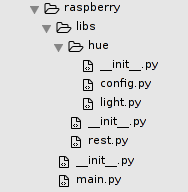
\includegraphics[width=0.35\textwidth]{dirs.png}
          \caption{Estructura de directorios y ficheros del software del nodo central.}
          \label{dirs}
        \end{figure}

\section{Elección de electrónica para la detección de alertas}
\label{sec:sistemas_interconexion}

    Teniendo en cuenta la facilidad que supone el uso de relés y la sencillez de su montaje electrónico e inclusión en el sistema, se opta por esta opción.

    \subsection{Detección de alertas del telefonillo}

    Para la detección de alertas por parte del telefonillo, se utiliza un relé de 12 Vac para detectar las llamadas. Este relé se conecta, por la toma de entrada, a la salida del telefonillo (la salida de su interruptor) y a corriente eléctrica de 12 Vac. La salida del relé se conecta al nodo central (la Raspberry Pi), conectando un extremo a un pin GND del GPIO (en concreto el pin 9 de la numeración física~\cite{raspberrypigpio}) y el otro, mediante resistencia de pull-up de 4,7 K$\Omega$, al pin 18 GPIO (de numeración GPIO) y a una salida de corriente de 3,3 V (pin 17 de la numeración física~\cite{raspberrypigpio}), tal como se observa en la figura~\ref{circuitotelefonillo}.\\

    \begin{figure}[!ht]
      \centering
        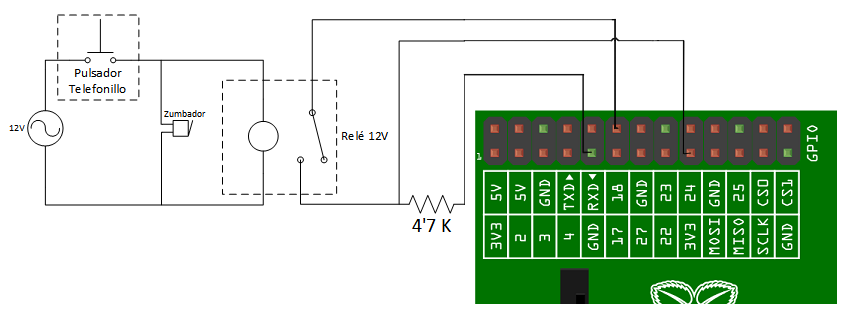
\includegraphics[width=0.75\textwidth]{circuitotelefonillo.png}
      \caption{Diseño del circuito de interconexión telefonillo-nodo central.}
      \label{circuitotelefonillo}
    \end{figure}
    
        \subsubsection{Implementación}
    
        Para la implementación de este circuito en el sistema, se crea una placa de circuito impreso (PCB) con los componentes y conexionado necesario. El esquemático y el diseño del layout de esta PCB se encuentran en el documento de Planos, en los planos número 1 (apartado~\ref{sec:plano1}) y número 2 (apartado~\ref{sec:plano2}), respectivamente. \\
        
        Teniendo en cuenta que el consumo del telefonillo no supera los 2 A de corriente, a un voltaje de 12 V, y utilizando una longitud de pistas de entrada al relé de 2 cm, se calcula que el ancho de las pistas que soporte esta tensión debe ser como mínimo de 780 $\mu$m. \\
        
        Por otro lado, al conectarse esta PCB a los pines GPIO de Raspberry Pi, que generan una corriente de 3,3 V a 50 mA~\cite{raspberry_pinout}, y suponiendo que estas placas de circuito impreso se sitúen a una distancia estimada de 30 m de la Raspberry Pi, utilizando cableado de 20 AWG de diámetro se obtendría una caída de voltaje de 51,35 mV (1,56 \%), lo que supone una caída de voltaje despreciable, obteniendo un voltaje final de entrada al pin GPIO de Raspberry Pi de 3,25 V.

    \subsection{Detección de alertas del timbre}

    Para la detección de las alertas producidas por llamadas al timbre, se utiliza un relé de 230 Vac. Este relé se conecta, por la toma de entrada, a la salida del timbre (la salida de su interruptor) y a corriente eléctrica de 230 Vac. A su vez, la salida del relé se conecta a la Raspberry Pi conectando un extremo a un pin GND del GPIO (en concreto el pin 6 de la numeración física~\cite{raspberrypigpio}) y el otro, mediante resistencia de pull-up de 4,7 K$\Omega$, al pin 17 GPIO (de numeración GPIO) y a una salida de corriente de 3,3 V (pin 1 de la numeración física~\cite{raspberrypigpio}), tal como se observa en la figura~\ref{circuitotimbre}.\\

    \begin{figure}[H]
      \centering
        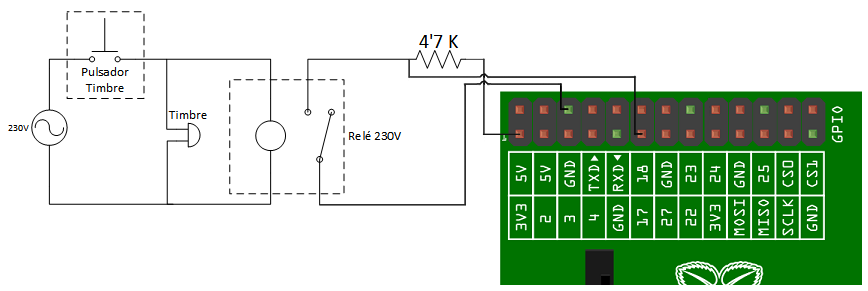
\includegraphics[width=0.8\textwidth]{circuitotimbre.png}
      \caption{Diseño del circuito de interconexión timbre-nodo central.}
      \label{circuitotimbre}
    \end{figure}
    
        \subsubsection{Implementación}

        Para la implementación de este circuito en el sistema, se crea una placa de circuito impreso (PCB) con los componentes y conexionado necesario. El esquemático y el diseño del layout de esta PCB se encuentran en el documento de Planos, en los planos número 3 (apartado~\ref{sec:plano3}) y número 4 (apartado~\ref{sec:plano4}), respectivamente. \\
        
        Teniendo en cuenta que el consumo del timbre no supera los 0,2 A de corriente, a un voltaje de 220 V, y utilizando una longitud de pistas de entrada al relé de 2,5 cm, se calcula que el ancho de las pistas que soporte esta tensión debe ser como mínimo de 32 $\mu$m. \\
        
        Por otro lado, el cálculo de caída de voltaje se realiza de la misma manera que para la placa anterior, y utilizando el mismo cableado resulta el mismo porcentaje de caída de voltaje, 1,56 \%, suponiendo que la entrada del telefonillo a la vivienda también se sitúe a 30 m de la Raspberry Pi y por tanto se ubique ahí esta placa de circuito impreso.
        
\section{Integración del sistema}

    Para la integración del sistema completo, el nodo central tendrá que comunicar con el resto de dispositivos y sistemas que conforman el sistema final, siendo el nodo central la Raspberry Pi, y los nodos subyacentes los sistemas de interconexión con el telefonillo y el timbre (de los que recibirá información el nodo central), el puente Philips Hue y el smartphone Android, con los que se comunicará a través del router integrado y se recibirá información además de enviar alertas hacia ellos. \\

    \begin{figure}[H]
      \centering
        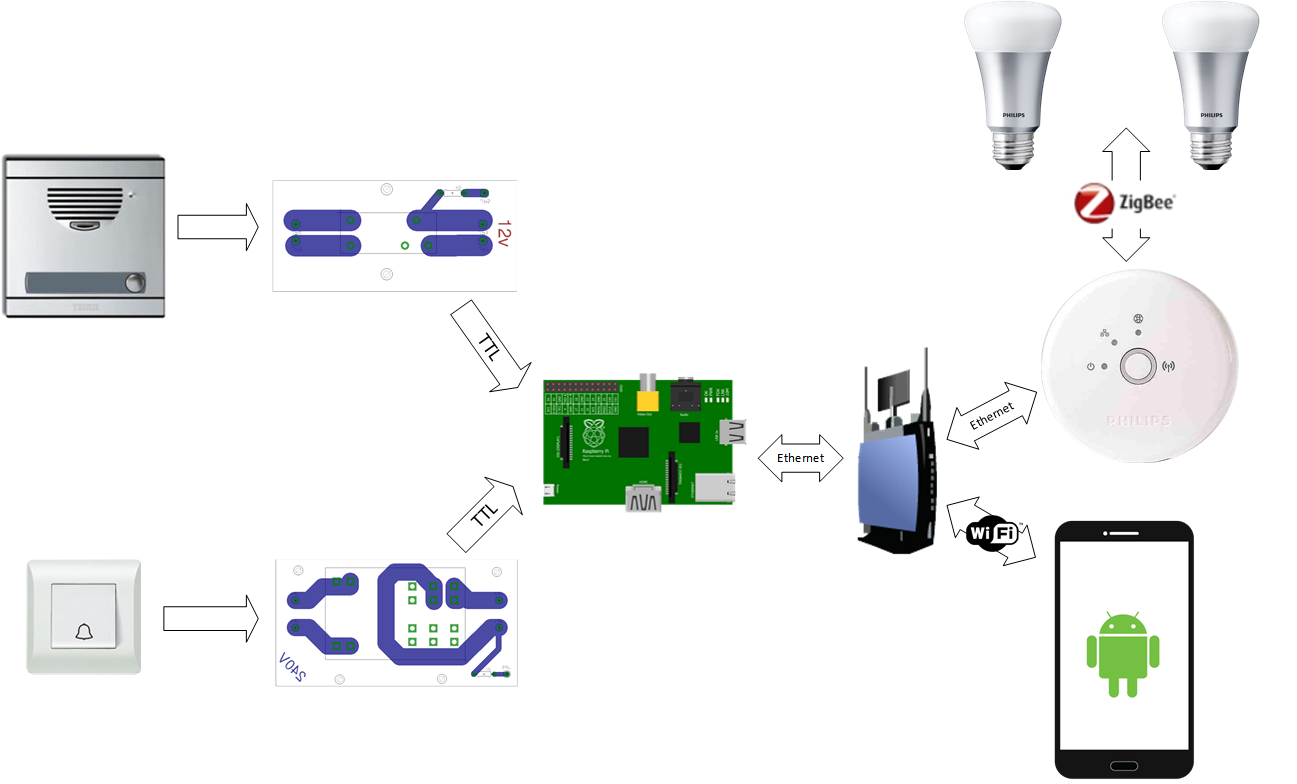
\includegraphics[width=0.9\textwidth]{integracion_sys.png}
      \caption{Diagrama de integración del sistema con el nodo central.}
      \label{integracion_sys}
    \end{figure}
    
     Complementando este diagrama, en la figura~\ref{diagrama_arquitectura} se puede observar el diseño final del sistema de forma detallada, incluyendo todos los elementos que lo conforman, una vez se ha definido el conexionado entre los sistemas de interconexión, el nodo central, el puente Philips Hue y el smartphone. \\

    \begin{figure}[H]
      \centering
        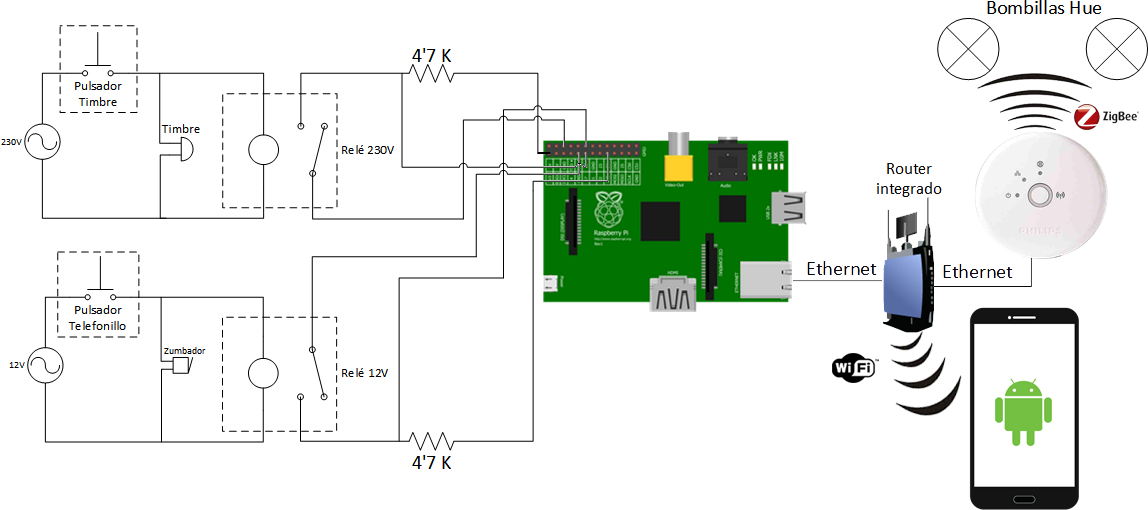
\includegraphics[width=1\textwidth]{diagrama_arquitectura.png}
      \caption{Diseño final de la arquitectura del sistema.}
      \label{diagrama_arquitectura}
    \end{figure}

\section{Aplicación para Android}

    \subsection{Diseño de la aplicación}

    El diseño de la aplicación sigue las normas de diseño de Google, utilizando una interfaz basada en MaterialDesign. Tras realizar un diseño de prototipo, el cual se puede observar en el apartado~\ref{sec:disenoapp}, previo al uso del IDE Android Studio, se decide basar el estilo general de la aplicación en el predeterminado generado por Android Studio al utilizar MaterialDesign como base. En cada pantalla de la aplicación se encuentra la barra superior de la aplicación, ActionBar, en la que se encuentra el acceso al menú de configuración o el botón de vuelta a la pantalla anterior, según la vista en la que se encuentre el usuario. En la figura~\ref{app1} se puede observar la pantalla principal de la aplicación. \\

    \begin{figure}[H]
      \centering
      {%
        \setlength{\fboxsep}{0pt}%
        \setlength{\fboxrule}{1pt}%
        \fbox{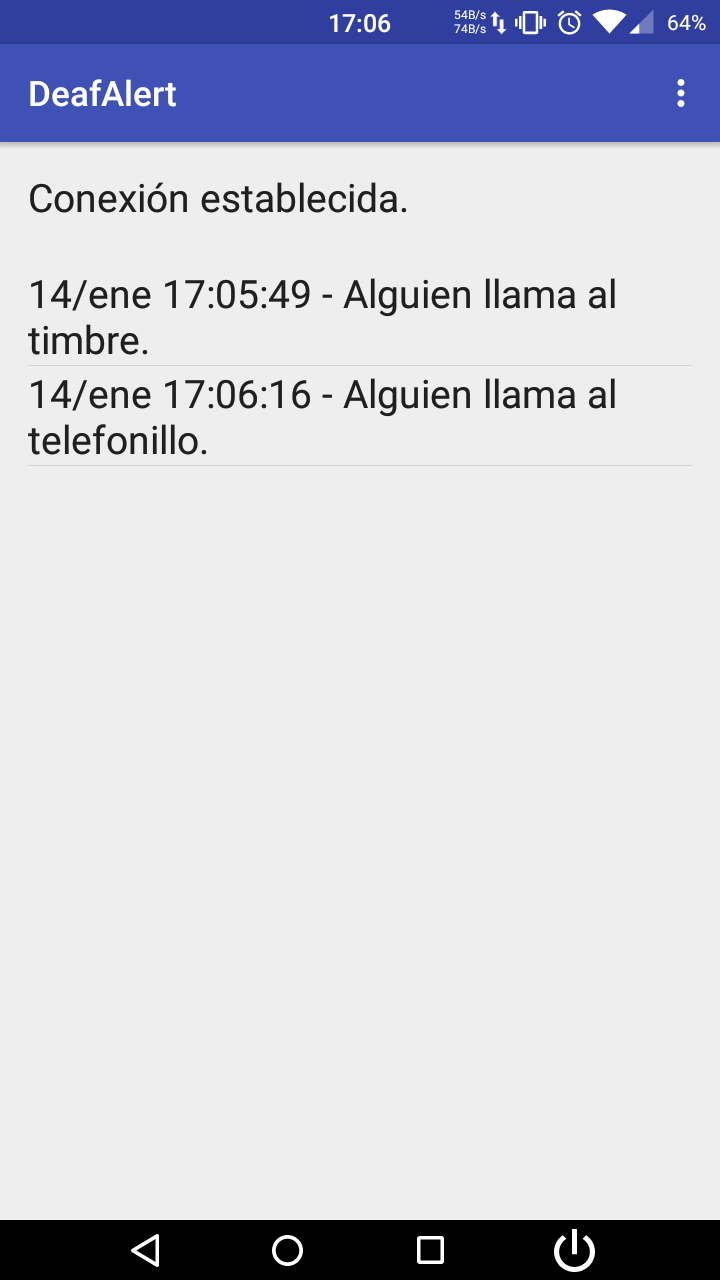
\includegraphics[width=0.3\textwidth]{app1.png}}
      }%
      \caption{Pantalla principal de la aplicación para Android.}
      \label{app1}
    \end{figure}

    En esta pantalla principal se encuentra la lista de alertas recibidas desde el servidor de alertas (la Raspberry Pi), además de un texto que indica el estado de conexión o de alertas entrantes. Tal como se muestra en la figura~\ref{app2}, estas alertas pueden ser eliminadas a mano desde la propia aplicación, de tal manera que cuando el usuario pulsa en una de ellas, la aplicación mostrará un mensaje preguntando si se desea eliminar la alerta. \\

    \begin{figure}[!ht]
      \centering
      {%
        \setlength{\fboxsep}{0pt}%
        \setlength{\fboxrule}{1pt}%
        \fbox{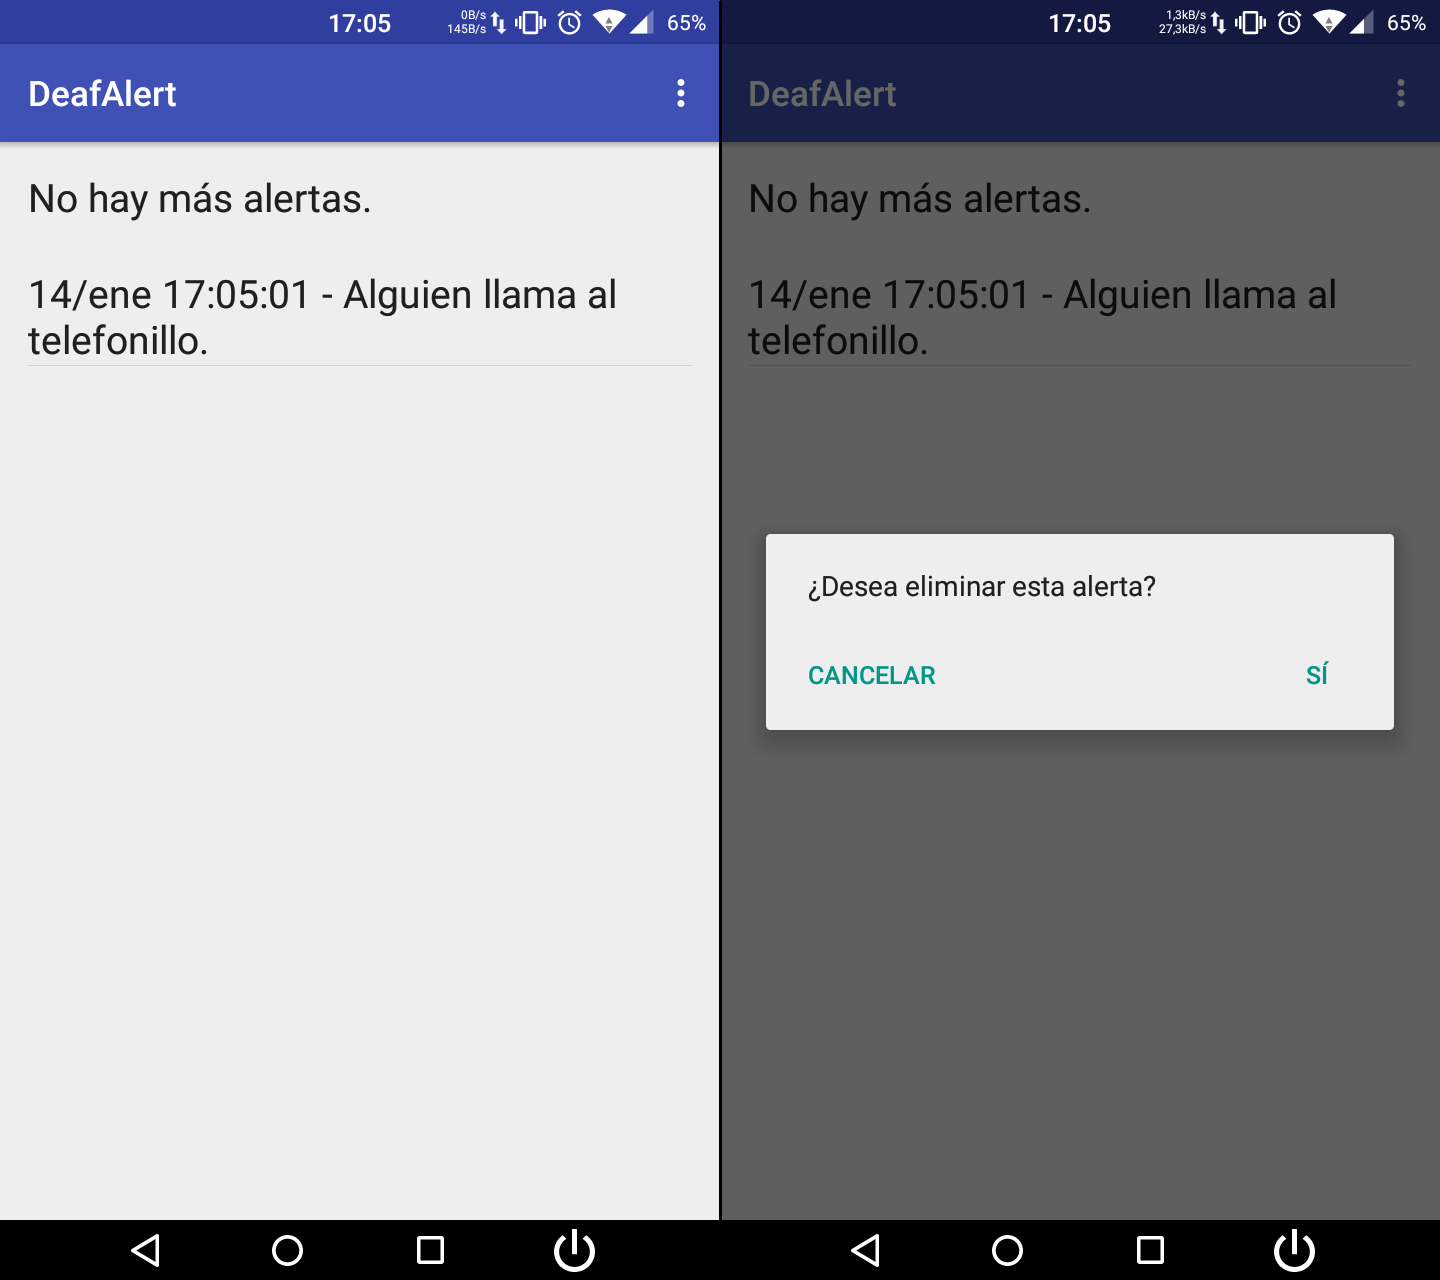
\includegraphics[width=0.6\textwidth]{app2.png}}
      }%
      \caption{Borrado de alertas en aplicación para Android.}
      \label{app2}
    \end{figure}

    Además de esta pantalla principal, la aplicación cuenta con un menú de configuración, fácilmente accesible mediante el menú desplegable superior, donde se puede configurar la dirección IP del servidor de alertas, tal y como se observa en la figura~\ref{app3}.

    \begin{figure}[H]
      \centering
      {%
        \setlength{\fboxsep}{0pt}%
        \setlength{\fboxrule}{1pt}%
        \fbox{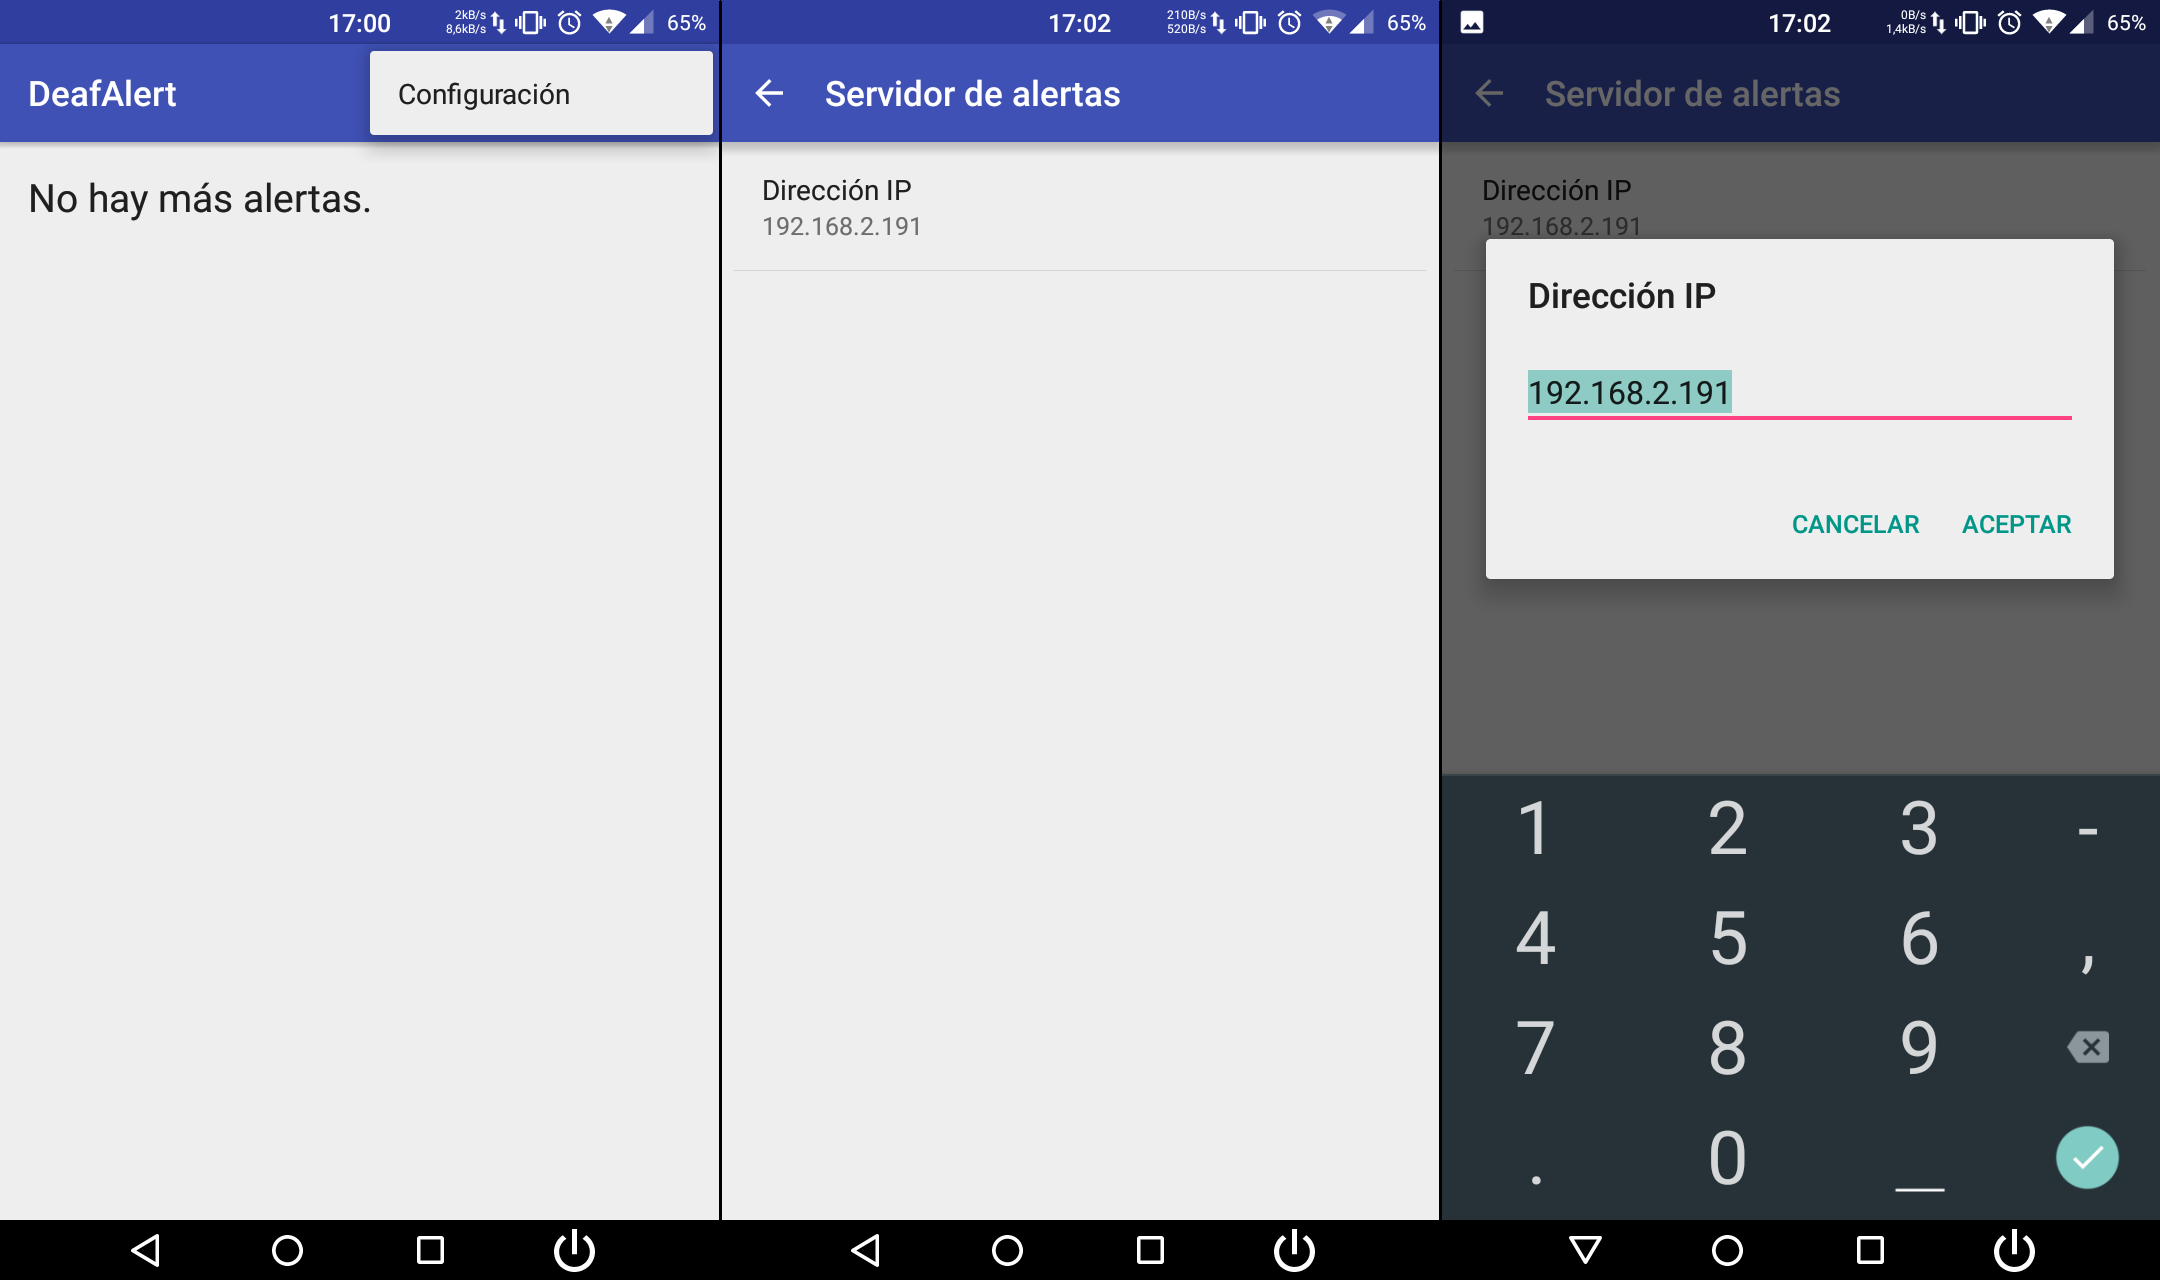
\includegraphics[width=0.8\textwidth]{app3.png}}
      }%
      \caption{Menú de configuración de aplicación para Android.}
      \label{app3}
    \end{figure}

    \subsection{Estructura software principal}

    La aplicación Android, desarrollada con el IDE Android Studio, se basa en tres clases java principales, divididas en archivos del mismo nombre:

    \begin{itemize}
        \item \textbf{MainActivity}: Clase principal de la aplicación, encargada de construir la vista principal de la aplicación Android, y dar funcionalidad a la misma. Es además la encargada de comunicar con el nodo central, tratar las alertas y mostrarlas en la pantalla principal.
        \item \textbf{AlertListAdapter}: Clase utilizada por MainActivity, para controlar la lista de alertas entrantes e ir refrescando la vista principal de la aplicación con esas alertas.
        \item \textbf{SettingsActivity}: Clase generada por el propio IDE, la cual implementa el menú de configuración de la aplicación, modificada para dotar a la aplicación de un menú de configuración que se adapte a las necesidades.
    \end{itemize}

    Además de estas clases java, la aplicación cuenta con otra clase java más generada por Android Studio, la cual no se analizará, pues es código generado automáticamente.

        \subsubsection{Actividad principal}

        En la actividad principal (MainActivity) es donde se desarrolla la funcionalidad principal de la aplicación, y es la encargada de generar la vista principal de la misma (la vista a la que se accede una vez se abre la aplicación).

        \androidexternal[linerange={35-68}]{./contenido/src/android/MainActivity.java}
        \vspace{0.3cm}

        Esta clase cuenta con varios atributos necesarios para almacenar la dirección IP del servidor de alertas, referencias a partes de la vista principal, una lista de cadenas que constituyen las alertas, un adaptador para estas alertas que será el encargado de refrescar las vistas, y otros atributos utilizados para control de notificaciones. \\

        La función principal de la clase y por tanto de la actividad es el método \textbf{onCreate}, el cual se encarga de dotar de funcionalidad a la aplicación cuando la vista principal es cargada. Además de inicializar algunos de los atributos anteriormente citados con valores predeterminados establecidos en la aplicación, se establece un objeto \textbf{AlertListAdapter} asociado a la actividad y a la lista de alertas. Una vez que esto está hecho, se crea un objeto de la clase Timer, el cual se encarga de ejecutar un método determinado cada cierto periodo de tiempo. Este método es \textbf{printRaspberryData}, el cual se examinará más adelante. \\

        Con todos los atributos inicializados y el Timer puesto en marcha, se establecen las políticas de la aplicación y se pone esta en funcionamiento. \\

        \androidexternal[linerange={124-125,147-209}]{./contenido/src/android/MainActivity.java}
        \vspace{0.3cm}

        El método \textbf{printRaspberryData} tiene un funcionamiento bastante sencillo, el cual se limita a establecer un objeto de tipo Runnable para el hilo principal de la interfaz de la aplicación. \\

        Es en este objeto Runnable donde se desarrolla el funcionamiento principal de la aplicación. En él se establece el comportamiento del método \textbf{run()}, método asociado a cada ejecución del hilo. Lo primero que realiza este método es comprobar la conexión WiFi del dispositivo. Si este no está habilitado, muestra un mensaje de error y sale del método, esperando a la próxima ejecución de este método a raíz del Timer establecido en \textbf{onCreate} para comprobar de nuevo si la conexión WiFi ha sido habilitada. \\

        Una vez el dispositivo cuente con conexión WiFi, se obtienen las preferencias almacenadas en el contenedor SharedPreferences de la aplicación. De estas preferencias se obtiene la dirección IP del servidor de alertas del que recibir las mismas. \\

        A continuación, se crea un objeto \textbf{DatagramSocket}, un socket de conexión UDP, el cual se configura para conectar a la dirección del servidor de alertas (la Raspberry Pi) a través del puerto 8080. Además se establece el puerto de escucha de datos entrantes en el puerto 8081. Si la conexión se lleva a cabo correctamente, se realiza una petición con el dato asociado ``GET /getAlert'', incluyendo este mensaje en un objeto \textbf{DatagramPacket}, paquete UDP que será enviado a través del socket. \\

        Si el envío surte efecto, se crea un nuevo objeto DatagramPacket, pero esta vez no será enviado, sino que servirá para almacenar los datos entrantes. A continuación, el hilo queda a la espera de alguna conexión entrante a través del socket. Una vez hay datos entrantes, el paquete se almacena en el objeto creado anteriormente, se extrae el dato (la alerta), y se añade a la lista de alertas, mostrándola por pantalla a través del objeto \textbf{AlertListAdapter}. Además, se muestra un mensaje de conexión satisfactoria en la aplicación, y si la aplicación estuviera en segundo plano o el dispositivo se encontrase en modo reposo (bloqueado), se envía una notificación al sistema con la alerta entrante. El comportamiento del objeto AlertListAdapter, así como lo que ocurre con la lista de alertas, se tratan en el apartado~\ref{sec:alertlistadapter}. \\

        \androidexternal[linerange={90-116}]{./contenido/src/android/MainActivity.java}
        \vspace{0.3cm}

        Además, en el método \textbf{onResume} se establece el comportamiento de la app cuando se pulse en alguna de las alertas de la lista, utilizando para ello el método \textbf{OnItemClickListener} de la clase AdapterView, el cual crea una instancia de un objeto de escucha de clicks en items o elementos de la lista. Redefiniendo el método \textbf{onItemClick} se establece este comportamiento. En primer lugar, se crea un objeto AlerDialog.Builder, el cual se encargará de generar un diálogo emergente de alerta. A continuación se establecen el mensaje del diálogo (mediante el método \textbf{setMessage}), la funcionalidad al pulsar el botón ``Cancelar'', el cual simplemente saldrá del diálogo de alerta, y la funcionalidad del botón ``Sí'', el cual eliminará la alerta de la lista. Finalmente, se genera el objeto de alerta y se muestra la alerta mediante el método \textbf{show}. \\

        \androidexternal[linerange={70-88}]{./contenido/src/android/MainActivity.java}
        \vspace{0.3cm}

        Por otro lado, mediante el método \textbf{onCreateOptionsMenu} se establece el menú de la aplicación, generando un botón para acceder al menú mediante el método \textbf{getMenuInflater}. \\

        Además, se dota de funcionalidad al menú con el método \textbf{onOptionsItemSelected}, donde se asocia cada elemento del menú con una actividad a iniciar (una nueva vista de la aplicación). Esto se realiza mediante el uso de objetos de la clase Intent, asociando en este caso una instancia de esta clase a la clase SettingsActivity, clase que implementa la actividad del menú, que se expone en el apartado~\ref{sec:menuapp}. A continuación, se inicia la actividad por medio de este objeto Intent. \\

        \androidexternal[linerange={126-146}]{./contenido/src/android/MainActivity.java}
        \vspace{0.3cm}

        Finalmente, el último método de la actividad principal, \textbf{notifyAlertToNotification}, utilizado en el hilo Runnable explicado anteriormente, es el encargado de generar y enviar notificaciones al sistema. Lo primero que se realiza en esta función es crear un objeto Builder de la clase NotificationCompat, el cual se inicializa con una serie de opciones para la notificación, como son el icono de la notificación, el título, el texto que debe contener, y distintos tipos de alerta como el color con el que el led del smartphone debe parpadear, la vibración, y cómo generar estas alertas. De este modo, la persona que utilice la aplicación podrá sentir mediante vibración o notar visualmente la alerta mediante el led, sin necesidad de tener el dispositivo desbloqueado. \\

        Tras crear este objeto, se crea una instancia de la clase Intent asociada a la actividad principal de la aplicación, y mediante un objeto de la clase TaskStackBuilder, se asigna el camino de vuelta al pulsar el botón ``Volver'' del propio dispositivo. A continuación, mediante un objeto de la clase NotificationManager se obtiene el servicio del sistema relacionado con las notificaciones, y se notifica la alerta mediante el método \textbf{notify} propio de esa clase, utilizando un número de identificación para la notificación, y el objeto builder creado al principio de la función.


        \subsubsection{Gestión de alertas}
        \label{sec:alertlistadapter}

        La gestión de las alertas a mostrar en la aplicación, así como la funcionalidad de refrescar las mismas en la lista de alertas dentro de la vista principal, se realiza mediante la clase \textbf{AlertListAdapter}, clase que hereda de la clase BaseAdapter, clase java de Android utilizada para actualizar el contenido de una vista ListView, vista utilizada en la vista principal para mostrar la lista de alertas. \\

        \androidexternal[linerange={15-23,69-72}]{./contenido/src/android/AlertListAdapter.java}
        \vspace{0.3cm}

        El constructor de la clase recibe un objeto Activity, la actividad asociada al Adapter, y un ArrayList de String, la lista de alertas. Mediante la instancia de Activity obtiene un objeto Inflater, necesario para obtener más adelante el objeto ListView a actualizar. \\

        Además, se crea una subclase ViewHolder, la cual incluye un objeto de tipo TextView, tipo utilizado para generar cada elemento de la lista ListView. \\

        \androidexternal[linerange={58-67}]{./contenido/src/android/AlertListAdapter.java}
        \vspace{0.3cm}

        Los métodos encargados de manipular la lista son \textbf{setData} y \textbf{remove}. El primero recibe una cadena con la alerta, la almacena en la lista, y mediante el método \textbf{notifyDataSetChanged} actualiza la información mostrada en la vista principal, refrescando el ListView asociado. El segundo método elimina un elemento de la lista y luego notifica de igual manera el cambio. \\

        \androidexternal[linerange={40-55}]{./contenido/src/android/AlertListAdapter.java}
        \vspace{0.3cm}

        Es necesario además sobrecargar el método \textbf{getView} de BaseAdapter, para poder obtener la vista a modificar cuando se deba actualizar el contenido de la lista de alertas. Este método usa un objeto de tipo View y otro de la subclase creada anteriormente, ViewHolder. Primero se obtiene el layout o vista a modificar de la apliación mediante el Inflater obtenido en el constructor, para a partir de esta referencia obtener la vista interna que actualizar, mediante su identificador. Hecho esto, ya se puede incluir el texto de la alerta en el TextView asociado al objeto ViewHolder utilizado.

        \subsubsection{Menú de configuración}
        \label{sec:menuapp}

        El menú de configuración está basado en el menú generado por Android Studio. Este menú incluye opciones sobrantes, por lo que se retiran todas las partes sobrantes dejando un único submenú con un campo de texto a rellenar, para configurar la dirección IP del servidor de alertas. \\

        Este menú se implementa mediante la clase SettingsActivity, el cual incluye subclases en su interior que heredan de la clase PreferenceFragment (propia del SDK de Android) por cada submenú. En este caso, al haber un único submenú, hay una única subclase, \textbf{ServerAlertsPreferenceFragment}. \\

        \androidexternal[linerange={141-168,179-179}]{./contenido/src/android/SettingsActivity.java}

        Esta clase cuenta con una constante de la clase Pattern, una plantilla, que define como debe estar formada una dirección IP, para poder comparar la preferencia establecida con esta plantilla, y así su validez. \\

        Es en el método \textbf{onCreate} donde se genera el campo para establecer la dirección IP. A continuación se genera una vista de texto para preferencias (EditTextPreference). Una vez hecho, se obtiene la preferencia con identificador \textbf{ip\_address}, y se establece una escucha para cuando el valor de esta preferencia cambie, con el método \textbf{setOnPreferenceChangeListener}. Como parámetro de este método, se crea un objeto \textbf{onPreferenceChangeListener}, para el cual se redefine la función onPreferenceChange. \\

        Esta función será la encargada de quedar a la espera de un cambio en el valor de la preferencia, comprobando cuando esto ocurra, si el valor es una dirección IP válida, mediante el método \textbf{matcher} de la clase Pattern. Finalmente, se almacena el valor de la preferencia mediante el método \textbf{bindPreferenceSummaryToValue}.
